% ----------
% A LaTeX template for course project reports
%
% This template is modified from "Tech Report ala MIT AI Lab (1981)"
%
% ----------
\documentclass[12pt, letterpaper, twoside]{article}
\usepackage{geometry}
\usepackage[utf8]{inputenc}
\usepackage[english]{babel}
\usepackage[runin]{abstract}
\usepackage{titling}
\usepackage{booktabs}
\usepackage{fancyhdr}
\usepackage{helvet}
\usepackage{csquotes}
\usepackage{graphicx}
\usepackage{blindtext}
\usepackage{parskip}
\usepackage{etoolbox}
\usepackage{amsmath}
\usepackage{float}
\usepackage{array}

% preamble.tex
\geometry{letterpaper, top=2.2in, headheight=1.7in}
\date{}

\makeatletter

\def\fulltitle#1{\def\@fulltitle{#1}}
\def\runningtitle#1{\def\@runningtitle{#1}}
\def\runningauthor#1{\def\@runningauthor{#1}}
\def\affiliation#1{\def\@affiliation{#1}}
\def\department#1{\def\@department{#1}}
\def\memoid#1{\def\@memoid{#1}}
\def\theyear#1{\def\@theyear{#1}}
\def\mydate#1{\def\@mydate{#1}}

\runningtitle{Course Project Report}
\author{Student Name}
\runningauthor{Student Name}
\affiliation{Kennesaw State University}
\department{College of Computing and Software Engineering}
\memoid{CS 4632 Project}
\theyear{2026}
\mydate{June 11, 2026}

\def\displaymydate{\@mydate}
\def\displaytheyear{\@theyear}
\def\displaymemoid{\@memoid}
\def\displaydepartment{\@department}
\def\displayaffiliation{\@affiliation}
\def\displayrunningauthor{\@runningauthor}
\def\displayrunningtitle{\@runningtitle}

\makeatother

\makeatletter
\patchcmd{\@zfancyhead}{\fancy@reset}{\f@nch@reset}{}{}
\patchcmd{\@set@em@up}{\f@ncyolh}{\f@nch@olh}{}{}
\patchcmd{\@set@em@up}{\f@ncyolh}{\f@nch@olh}{}{}
\patchcmd{\@set@em@up}{\f@ncyorh}{\f@nch@orh}{}{}
\makeatother

\pagestyle{fancy}
\renewcommand{\headrulewidth}{0pt}

\fancypagestyle{firstpage}
{
    \fancyhf{}
    \fancyhead{%
        \begin{center}
            \textsc{\displayaffiliation}\\
            \textsc{\displaydepartment}
        \end{center}
        \vspace*{0.5in}
        \displaymemoid
        \hfill
        \displaymydate
    }
    \fancyfoot[L]{\footnotesize \textbf{\textsc{\displayaffiliation} -- \displaytheyear}}
}
\fancyhead[EL]{\small \displayrunningauthor}
\fancyhead[ER]{\small Page \thepage}
\fancyhead[OL]{\small Page \thepage}
\fancyhead[OR]{\small \displayrunningtitle}

\chead{}
\lfoot{}
\cfoot{}
\rfoot{}

\providecommand{\keywords}[1]{\noindent \textbf{Keywords:} #1}

\renewcommand{\familydefault}{\sfdefault}
\setlength{\parskip}{0.7em}
\setlength{\parindent}{0pt}
\abslabeldelim{:}
\setlength{\abstitleskip}{-\absparindent}

\pretitle{\Large \begin{center}}
\posttitle{\\[2ex] \Large \textbf{by}\end{center}}




\title{\textbf{CS 4632 Course Project:\\
Discrete-Event Simulation of an Electronics Repair Department}}
\runningtitle{Electronics Repair Simulation}
\author{Carlos Guerrero}
\runningauthor{Carlos Guerrero}
\affiliation{Kennesaw State University}
\department{College of Computing and Software Engineering\\
CS 4632 -- Modeling and Simulation, Section W01}
\memoid{Milestone 5: Final Report}
\theyear{2026}
\mydate{July 23, 2026}


\begin{document}
\maketitle

\begin{abstract}
    \noindent
    This project is a discrete-event simulation of the electronics repair support
    department where I work. The department repairs printed circuit boards and
    HVAC/refrigeration controllers. Jobs arrive from advance exchanges, production-line
    failures, reships, and customer Return Material Authorizations (RMAs). I built the
    model in Python using SimPy, representing general and specialty technicians and test
    stations as preemptible resources, business-hours scheduling, and a priority
    queue where production, advance-exchange, and reship work can interrupt a customer RMA
    repair in progress. Using historical arrival and repair-time data, I ran a sensitivity
    analysis across nine parameters, compared ten scenarios, and validated the model. 
    The results show that resources are the department's real bottleneck, since adding technicians and stations 
    cut wait time by 97 to 99 percent, but that Customer RMA volume is what determines how far that fix can go:
    doubling it wiped out most of the benefit of also doubling every resource.

\end{abstract}

\vspace{1cm}

\noindent
\textbf{Project repository:}\\
\texttt{https://github.com/CarlosG100/CS4632-Electronics-Repair}

\thispagestyle{firstpage}

\pagebreak

\tableofcontents


\pagebreak

% ----------
% End of first page
% ----------

\newgeometry{}

\section{Introduction}
\label{sec:introduction}

The project is based on an electronics manufacturing support department. The department
receives PCBs and complete controller units, analyzes the failures, repairs what it can,
and records a final outcome. The workload is not constant because jobs arrive at
different times and repairs do not all take a uniform amount of time.

The main problem this project addresses is deciding how priority rules and limited
resources affect the different job types. Urgent production failures need a fast
response, but interrupting another repair increases the delay for normal customer work.
A simulation is useful here because the system changes over time and includes random
arrivals and repair times that cannot be captured by a single formula.

The project set out to answer three questions:

\begin{enumerate}
    \item How do first-in, first-out (FIFO) and priority with or without preemption affect turnaround time?
    \item How do technician specialization and station compatibility affect waiting and capacity?
    \item What practical change improves urgent response without creating a large RMA backlog?
\end{enumerate}

To answer these questions, I built a working simulation of the department, ran a
sensitivity analysis and a set of comparison scenarios against it, and validated the
model. 

\section{Background and Literature Review}
\label{sec:literature}

Five sources shaped the design of this project.

Banks et al. explain discrete-event simulation through entities, queues, resources,
events, and next-event time advance \cite{banks2005}. They also identify electronics
assembly operations as a manufacturing use of simulation. This matched my project because
controller and PCB jobs wait for limited resources, receive service, and leave with an
outcome. I adapted the basic service-system structure by adding four job sources,
compatible technician/station resources, business hours, and interruptions.

Law explains process-interaction simulation as following an entity through each step of a
system \cite{law2015}. This fit my project because each job moves through arrival,
waiting, service, and completion. I used Law's methods to build random inputs from
historical data, run each scenario as multiple independent replications, and compare
results using confidence intervals rather than single runs.

Cobham shows that priority service reduces the waiting time of high-priority work at the
cost of increasing the wait for lower-priority work \cite{cobham1954}. This was the main
tradeoff in the finished model. Production, advance-exchange, and reship work are served
ahead of a Customer RMA repair already in progress. I adapted the priority model by
updating what M1 originally scoped as four priority tiers into two: Customer RMA
work at one level, and every other source sharing a higher level, since in practice the
department does not treat AdvEx, reship, and production failures as different priorities
from one another.

Little proves the relationship $L = \lambda W$ between the average number of items in a
system, the throughput rate, and the average time in the system \cite{little1961}. An
important part of the result is that it does not depend on one specific arrival
distribution or queue discipline. 

Borshchev explains that service systems may require particular workers and shared
equipment \cite{borshchev2020}. This supported modeling the roughly 20 percent of jobs
that need a specialized technician and station. He also warns that adding every
real-world detail can make a model too large to manage. I kept individual technician
efficiency, parts inventory, equipment downtime, and rework outside the model for this simulation.

Finally, the simulation itself was built with SimPy, a Python discrete-event simulation
library, which supplied the event scheduling, resource, and interrupt primitives.

\section{Model Design and Architecture}

\subsection{Conceptual Model}

The entities are the jobs that flow through the department. Each job carries a source
(Customer RMA, Advance Exchange, Reship, or Production Failure), a priority, a required
capability (general or specialty), an arrival time, and a service time drawn from
historical data. Technicians and test stations are the department's limited passive
resources; each active repair uses one technician and one compatible station.

\subsection{UML Diagrams}

\begin{figure}[H]
\centering

\includegraphics[width=\textwidth]{class_diagram.png}
\caption{Classes and functions used by a live simulation run.}
\end{figure}

The M1 class diagram planned a single \texttt{RepairDepartment} class with
\texttt{start()}, \texttt{createJob()}, and \texttt{returnRMA()} methods, and a
\texttt{Repair} class that would manage an RMA rack and hand out resources. The finished
program did not turn out that way. \texttt{Job}, \texttt{Technician}, \texttt{Station},
\texttt{ScenarioConfig}, and \texttt{SimulationMetrics} are still data classes, but
the actual logic lives inside \texttt{simpy\_runner.py}
(\texttt{repair\_job()}, the arrival processes for each job source, and
\texttt{run\_basic\_fifo\_simulation()}). These functions work directly with four SimPy
\texttt{PreemptiveResource} pools, one each for general and specialty technicians and
general and specialty stations, instead of a custom \texttt{Repair} class.

\begin{figure}[H]
\centering

\includegraphics[width=\textwidth, height=8.5in, keepaspectratio]{activity_diagram.png}
\caption{Activity diagram for a job moving through arrival, technician selection, station selection, service, and possible interruption.}
\label{fig:activity-diagram}
\end{figure}

The M1 activity diagram showed Customer RMAs waiting on a physical rack, with only
production failures able to interrupt work already in progress. Both of these changed.
All four job sources are now generated as live SimPy processes instead of a pre-loaded
rack, and any non-RMA source (AdvEx, Reship, or Production) can interrupt a Customer RMA
repair, not just production failures. Figure~\ref{fig:activity-diagram} also shows a
borrowing rule that was not part of the M1 plan. A general job may use an idle specialty
technician or station when the general pool is busy. While it is borrowing, that job is
requested at the highest priority so another job cannot bump it off the resource it
borrowed.

\subsection{Key Design Decisions}

\begin{itemize}
    \item \textbf{Two priority levels} Customer RMA work is priority level
    1. AdvEx, Reship, and Production Failure all share priority level 0. This reflects how
    the real department treats these three sources as equally urgent relative to a
    standing customer repair. A Customer RMA request is also never allowed to preempt
    another job, no matter what the priority numbers say, since only AdvEx, Reship, and
    Production requests are given permission to preempt. In practice this means
    preemption only ever flows one direction: a non-RMA job can interrupt an in-progress
    RMA repair, but nothing interrupts a non-RMA job.
    \item \textbf{Resource overflow.} General-capability jobs may borrow
    an idle specialty resource; specialty-capability jobs may never use a general
    resource.
    \item \textbf{Business hours.} The simulation clock runs continuously, but repair work
    only advances between 7:00 AM and 3:30 PM, Monday through Friday. A job in progress at
    the end of a business day keeps its remaining time and resumes at the next business
    start.
    \item \textbf{Period-based job counts.} Instead of a fixed job count per scenario, job
    counts for each source are derived from a chosen simulated period (in hours) and that
    source's historical interarrival rate, so changing the simulated period automatically
    scales demand.
\end{itemize}

\section{Implementation}
\label{sec:implementation}

\subsection{Technologies Used}

The simulation is written in Python 3 using SimPy for event scheduling,
resources, and interrupts. Results are exported to CSV for analysis in microsoft excel.

\subsection{Core Algorithms}

Each job is handled by one process function, \texttt{repair\_job()}, that repeats until
the job is finished. Every pass through it does the same four things:

\begin{itemize}
    \item Checks whether the simulation clock is inside business hours, and waits until
    the next business day starts if not.
    \item Picks a technician and a station.
    \item Requests both resources at the right priority.
    \item Once both are assigned, works the job in chunks no longer than the hours left in
    the current business day, pausing overnight if the job is not finished by the end of
    the day.
\end{itemize}

If a higher-priority job preempts the resource in the middle of a repair, SimPy raises an
interrupt. The process then records whether the job had already started (an
``interrupted'' event) or was bumped before it ever started (a ``bumped'' event), and
loops back to try again. This is how the ``keep remaining time and rejoin the queue''
behavior from M1 actually works in the finished code.

\subsection{Data Structures}

\texttt{Job}, \texttt{Technician}, and \texttt{Station} are data classes holding
identity, capability, and timing fields. \texttt{ScenarioConfig} holds every tunable
parameter for a run (resource counts, simulated period, job counts, random seed,
preemption on/off). \texttt{SimulationMetrics} accumulates the event log, completed-job
records, and periodic queue snapshots taken during the run, and exports all three to CSV.

\subsection{Challenges Overcome}

\begin{itemize}
    \item \textbf{Learning SimPy (M2).} SimPy was a new library, and the biggest early
    hurdle was learning how its event scheduling and processes actually worked before
    writing any real simulation code. The first version of the job-selection logic was
    built without SimPy at all, as a proof of concept, and was reworked into SimPy only
    after that logic was confirmed to work.

    \item \textbf{Reship-hours discrepancy (M3).} While reviewing the \texttt{master
    index} and \texttt{config} outputs, the simulated hours for reship jobs
    did not line up with what the rest of the run was reporting. Debugging showed the reship interarrival time was being calculated incorrectly, and
    that the real interval between reship arrivals was more spread out than expected.

    \item \textbf{Overflow bug (M4).} While preparing the M4 parameter
    analysis, specialty technicians and stations turned out to be assigned only specialty
    jobs, even though the intended rule was that general jobs could borrow an idle
    specialty resource. Every scenario before this fix had specialty resources sitting
    idle whenever no specialty job was waiting, which understated how much specialty
    capacity actually helped.

    \item \textbf{Sparse historical data for reships.} Reship jobs are not logged in the
    department's real data. Based on personal experience working in the department,
    reship jobs were modeled using the same arrival rate as Advance Exchanges.
\end{itemize}

\section{Experimental Setup}
\label{sec:setup}

\subsection{Simulation Parameters}

The baseline configuration uses one general and one specialty technician, one general and
one specialty test station, preemption enabled, and job counts derived automatically from
a chosen simulation period using each source's historical interarrival rate.

\subsection{Scenarios Tested}

Ten scenarios were tested, varying resource counts, preemption, and demand volume.
Table~\ref{tab:scenarios} lists each one and what it was meant to test.

\begin{table}[H]
\centering
\caption{The ten scenarios tested, each run once against the baseline.}
\label{tab:scenarios}
\small
\begin{tabular}{p{3.3in} p{2.2in}}
\toprule
\textbf{Scenario} & \textbf{Purpose} \\
\midrule
Baseline & Default configuration \\
Extra Gen Tech/Station & Extra general technician \\
Extra Spec Tech/Station & Extra specialty technician \\
Extra Gen/Spec Tech/Station & Extra general station \\
Extra Gen/Spec Tech/Station and doubled Customer RMAs & Extra specialty station \\
100\% increase in all & Extra of everything \\
100\% w/ no preemption & No preemption \\
No preemption and extra spec & No preemption plus extra specialty tech \\
100\% increase in direct jobs with no preemption & Higher job volume \\
100\% increase in direct jobs with preemption & Higher job volume plus extra resources \\
\bottomrule
\end{tabular}
\end{table}

Figure~\ref{fig:run-summary} shows \texttt{run\_all\_scenarios.py} executing from the
command line. This run used the tool's default scenario definitions.

\begin{figure}[H]
\centering
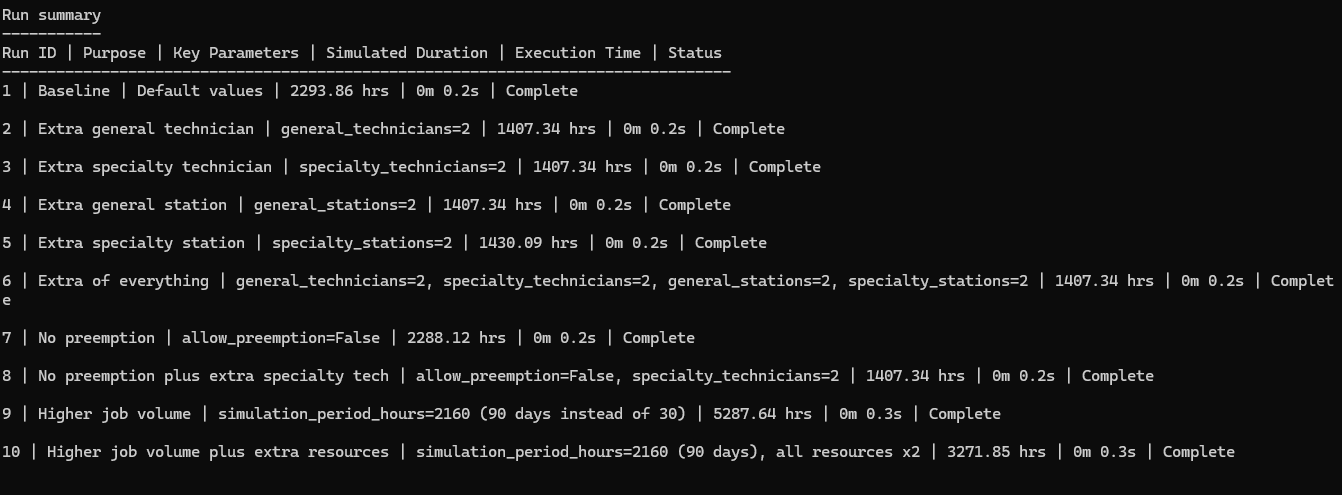
\includegraphics[width=\textwidth]{run_summary.png}
\caption{Terminal output from running \texttt{run\_all\_scenarios.py} with its default scenario definitions.}
\label{fig:run-summary}
\end{figure}

\subsection{Data Collection Methods}

Each run exports four CSV files: \texttt{events.csv} (a full event trace: arrivals,
starts, pauses, interruptions, completions), \texttt{summary.csv} (per-scenario
metrics and utilization), \texttt{config.csv} (the exact parameters used), and
\texttt{time.csv} (periodic queue-length and busy/idle snapshots).

\subsection{Experimental Design}

Analysis tools were built on top of the base simulation. \texttt{parameterUpdate.py}
runs a baseline and then one or more single-parameter changes, each averaged over 100
replications with a fixed set of random seeds shared across every parameter value, 
so that differences in the output can be attributed to the
parameter change rather than randomness. \texttt{replicate.py} runs one configuration
for 100 replications with independent random seeds and reports the mean, standard
deviation, min, max, and 95\% confidence interval for wait time, turnaround time, and
throughput.

\section{Results and Analysis}
\label{sec:results}

\subsection{Sensitivity Analysis}

Nine parameters were each increased by 100 percent from baseline and run for 100
replications. Table~\ref{tab:sensitivity} reports the sensitivity ratio
for wait time and turnaround time on each one.

\begin{table}[H]
\centering
\caption{Sensitivity of average wait time and turnaround time to a 100\% increase in each parameter.}
\label{tab:sensitivity}
\small
\begin{tabular}{lrrr}
\toprule
\textbf{Parameter} & \textbf{New Value} & \textbf{Wait Sensitivity} & \textbf{Turnaround Sensitivity} \\
\midrule
General technicians & 2 & -0.348 & -0.312 \\
General stations & 2 & -0.377 & -0.342 \\
Specialty technicians & 2 & -0.260 & -0.220 \\
Specialty stations & 2 & -0.332 & -0.302 \\
Simulation period (hrs) & 1440 & 1.403 & 1.302 \\
Customer RMA jobs & 56 & 0.856 & 0.814 \\
AdvEx jobs & 16 & 0.051 & 0.047 \\
Reship jobs & 16 & 0.045 & 0.035 \\
Production jobs & 38 & -0.021 & -0.040 \\
\bottomrule
\end{tabular}
\end{table}

\begin{figure}[H]
\centering
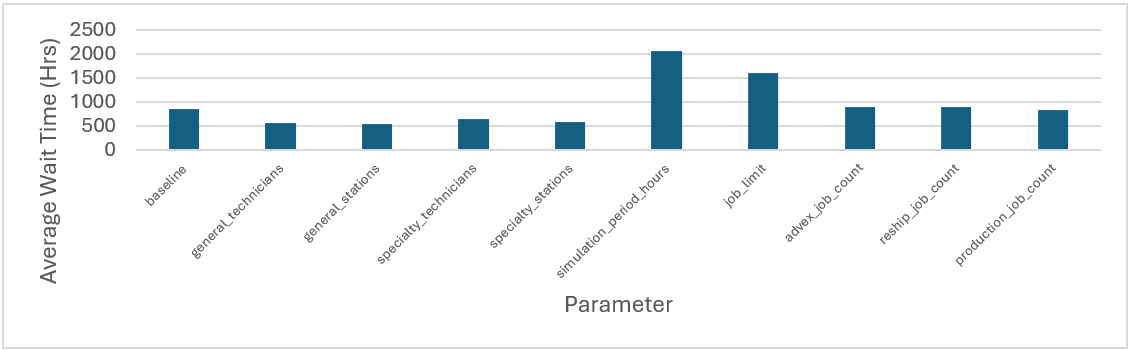
\includegraphics[width=\textwidth]{sensitivity_chart.png}
\caption{Average wait time after a 100\% increase in each parameter. Customer RMA volume
(\texttt{job\_limit}) and simulation period, which scales Customer RMA volume along with
every other source, produce far more wait time than any resource increase or any other
demand source.}
\label{fig:sensitivity-chart}
\end{figure}

Customer RMA job volume was the dominant driver of wait time. Doubling the Customer RMA
job count alone had a sensitivity of 0.856, while doubling AdvEx, Reship, or Production
volume individually had almost no effect. Doubling the simulation period had the largest
sensitivity of all (1.403), but that is really the same RMA effect showing up twice. A
longer period increases every source's job count together, including Customer RMA.
Adding technicians or stations of any type reduced wait time, but by a smaller amount
than RMA volume increased it.

\subsection{Scenario Comparison}

Table~\ref{tab:scenario-results} shows the results for the ten scenarios listed in
Table~\ref{tab:scenarios}. Scenarios that
raise Customer RMA demand push wait time up by close to two times compared
to baseline, while scenarios that only add technicians or stations bring wait time down,
but by a much smaller amount.

\begin{table}[H]
\centering
\caption{Average wait time, turnaround time, and throughput for each scenario.}
\label{tab:scenario-results}
\small
\begin{tabular}{p{2.2in} >{\raggedleft\arraybackslash}p{0.85in} >{\raggedleft\arraybackslash}p{0.95in} >{\raggedleft\arraybackslash}p{0.95in}}
\toprule
\textbf{Scenario} & \textbf{Avg Wait (hrs)} & \textbf{Avg Turnaround (hrs)} & \textbf{Throughput (jobs/hr)} \\
\midrule
Baseline & 780.24 & 816.95 & 0.0275 \\
Extra Gen Tech/Station & 18.17 & 53.05 & 0.0448 \\
Extra Spec Tech/Station & 2.06 & 37.96 & 0.0448 \\
Extra Gen/Spec Tech/Station & 8.00 & 41.92 & 0.0448 \\
Extra Gen/Spec Tech/Station, doubled RMAs & 92.01 & 174.02 & 0.0242 \\
100\% increase in all & 0.65 & 29.27 & 0.0534 \\
100\% w/ no preemption & 7.72 & 37.20 & 0.0534 \\
No preemption and extra spec & 1.89 & 36.27 & 0.0448 \\
100\% increase in direct jobs, no preemption & 844.68 & 869.09 & 0.0411 \\
100\% increase in direct jobs, with preemption & 845.56 & 870.20 & 0.0410 \\
\bottomrule
\end{tabular}
\end{table}

\begin{figure}[H]
\centering
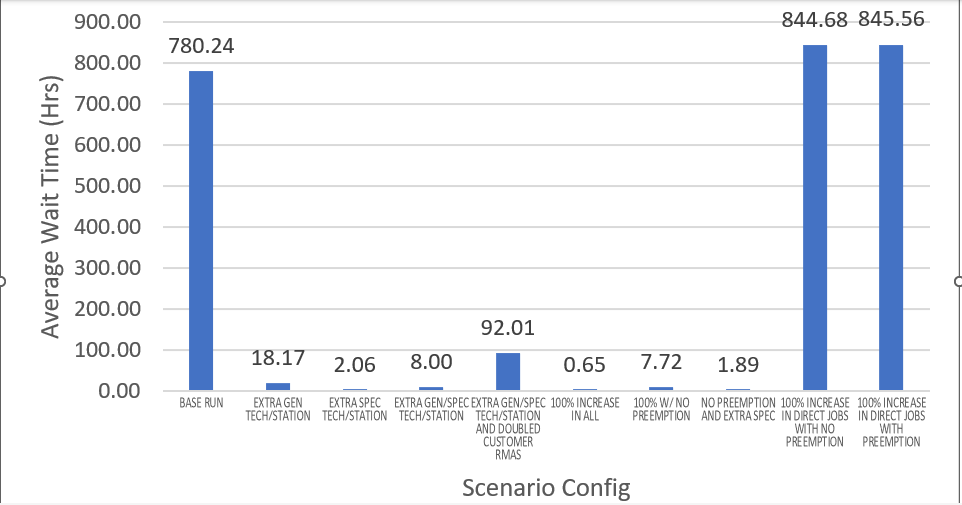
\includegraphics[width=\textwidth]{scenario_chart.png}
\caption{Average wait time by scenario. Scenarios that raise Customer RMA demand push
wait time up by close to two times compared to baseline, while scenarios
that only add technicians or stations bring wait time down by a much smaller amount.}
\label{fig:scenario-chart}
\end{figure}

The two scenarios with the smallest wait times were the ones that added resources to 
handle customer RMA demand. The two worst scenarios both doubled direct-request volume (AdvEx,
Reship, and Production together) while leaving Customer RMA demand and staffing
unchanged, and preemption made almost no difference between them (845.56 hours with
preemption versus 844.68 without). Turning
preemption on or off barely moved the average wait time in this scenario, which shows
that once the department is working at capacity, preemption stop mattering much
compared to raw demand.

\subsection{Statistical Summary}

\begin{table}[H]
\centering
\caption{Statistical summary across 100 replications, baseline configuration.}
\label{tab:stats-baseline}
\begin{tabular}{p{2.0in} >{\raggedleft\arraybackslash}p{0.7in} >{\raggedleft\arraybackslash}p{0.7in} >{\raggedleft\arraybackslash}p{0.85in} >{\raggedleft\arraybackslash}p{0.85in}}
\toprule
\textbf{Metric} & \textbf{Mean} & \textbf{Std Dev} & \textbf{95\% CI Lower} & \textbf{95\% CI Upper} \\
\midrule
Average wait time (hrs) & 982.65 & 1459.89 & 696.51 & 1268.79 \\
Average turnaround time (hrs) & 1080.33 & 1540.82 & 778.32 & 1382.33 \\
Throughput (jobs/hr) & 0.0251 & 0.0182 & 0.0216 & 0.0287 \\
\bottomrule
\end{tabular}
\end{table}


\begin{table}[H]
\centering
\caption{Statistical summary across 100 replications, baseline vs. one added specialty technician.}
\label{tab:stats-contrast}
\begin{tabular}{p{2.2in} >{\raggedleft\arraybackslash}p{0.65in} >{\raggedleft\arraybackslash}p{0.65in} >{\raggedleft\arraybackslash}p{0.8in} >{\raggedleft\arraybackslash}p{0.8in}}
\toprule
\textbf{Configuration / Metric} & \textbf{Mean} & \textbf{Std Dev} & \textbf{95\% CI Lower} & \textbf{95\% CI Upper} \\
\midrule
Baseline -- avg wait (hrs) & 927.19 & 1612.64 & 611.12 & 1243.27 \\
+1 Specialty Tech  & 703.28 & 1348.88 & 438.90 & 967.66 \\
\addlinespace
Baseline -- avg turnaround (hrs) & 1023.51 & 1692.22 & 691.84 & 1355.19 \\
+1 Specialty Tech  & 812.31 & 1481.32 & 521.97 & 1102.65 \\
\addlinespace
Baseline -- throughput (jobs/hr) & 0.0269 & 0.0176 & 0.0234 & 0.0303 \\
+1 Specialty Tech  (jobs/hr) & 0.0277 & 0.0189 & 0.0240 & 0.0314 \\
\bottomrule
\end{tabular}
\end{table}

Adding a specialty technician lowered mean wait time by about 24 percent and mean
turnaround time by about 21 percent. The two 95\% confidence intervals only overlap
partially. This replication only added a second specialty technician and left specialty stations at one, so the station
stayed a constraint even though the technician did not. Adding one resource but not the other does not fully relieve the stress of lack of resources for demand.

\section{Validation and Verification}
\label{sec:validation}

\texttt{validate\_simulation.py} runs a set of
automated checks against simulation runs (resource release, non-negative remaining
time, event ordering) as code-level verification. 

Validation approaches used:

\textbf{Face validation.} In a real repair department, wait times and queues should grow
and shrink with resource availability, and that is what the simulation shows. Adding
general technicians and stations produced a large improvement in wait time and queue
length, and adding specialty technicians and stations instead produced an even bigger
improvement, since specialty resources can work both general and specialty jobs.
Wait times and queue length grow again once demand is increased past what the added
resources can handle.

\textbf{Parameter validation.} The simulation's inputs come from the department's real
historical data, cleaned of any company or customer information. That data was used to
find the average arrival rate, service time, general/specialty split, outcome, and
priority for each job source. The one exception is reships, which are not logged in the
real data. Based on my personal experience working in the department, reship jobs were
given the same rates as Advance Exchanges, since they arrive and get handled in a
similar way. This is the simulation's biggest weakness as it is an estimate from my experience instead of being built
on averages from hard data.

\section{Discussion}
\label{sec:discussion}

Returning to the three research questions from Section~\ref{sec:introduction}:

\textbf{FIFO and priority with or without preemption.} The scenario data has two clean
comparisons where preemption is the only thing that changes. At doubled resources and
doubled demand, average wait time was 0.65 hours with preemption on and 7.72 hours with
it off, roughly ten times increase. At baseline resources with only direct-request demand
doubled and Customer RMA demand unchanged, average wait time was 845.56 hours with
preemption on and 844.68 hours with it off, almost no difference. Preemption helps
when the system still has enough capacity to assign resources. Once
the system is at capacity, whether an urgent job can interrupt another job barely
matters.

\textbf{Technician specialization and station compatibility.} At baseline demand, adding one general technician and station
dropped wait time by about 97 percent (Table~\ref{tab:scenario-results}), and adding one
specialty technician and station instead dropped it by about 99 percent, since specialty
resources can also work general jobs while general resources cannot work specialty jobs.
Specialty capability compatibility is what makes the extra resource worth more than
a general resource.

\textbf{Practical change} Based on both the
sensitivity analysis and the scenario comparison, adding a specialty technician and
station is the single change that helped the most. It fixes the bottleneck directly
instead of just protecting urgent work at the expense of Customer RMAs.
Table~\ref{tab:scenario-results} shows the limit of that fix.
Doubling Customer RMA demand on top of doubled resources pushed wait time from about 8
hours back up to about 92 hours, erasing the benefits of more resources. Adding resources is the
right move, but it stops working if Customer RMA demand keeps growing.

\section{Conclusion and Future Work}
\label{sec:conclusion}

This project built a discrete-event simulation of the repair department's technician and
station resources, tested it against nine parameters and ten scenarios, and validated it.
The main conclusion is that resources are the bottleneck in this
department. Adding a general technician and station dropped wait time by about 97
percent, and adding a specialty technician and station instead dropped it by about 99
percent, since specialty resources can also cover general work. Preemption did not make
a meaningful difference once resources were already running at capacity
(Section~\ref{sec:discussion}). Customer RMA demand is the parameter that puts the most
stress on the department. Doubling it erased most of the benefit of also doubling
every resource. It took wait time from about 8 hours back up to about 92 hours. The best
scenario tested was adding one specialty technician and station at normal demand, with
a wait time around 2 hours and a turnaround time around 38 hours. The worst was baseline
resources with higher Customer RMA demand. If the department changed one thing, adding
more specialty technicians and stations would be the recommendation, since it was the
biggest single contributor to lower wait and turnaround times in every scenario tested.

This project's main weakness is the reship interarrival rate, which relies on a
personal experience estimate rather than historical data. Another weakness is the assumption that repair
times reflect a consistent human work pace without modeling individual technician
efficiency, parts delays, equipment downtime, or rework. Future work could add
technician-level efficiency variation, a parts-availability delay for advance exchanges.

% ----------
% Bibliography
% ----------

\bibliography{references}
\bibliographystyle{abbrv}

\end{document}

% ----------
